\section{Method}

\subsection{Machine learning pipeline}
To solve the problem of anomaly detection and image classification, a machine learning pipeline has been developed. The pipeline consists of a anomaly detection procedure that use an autoencoder to reconstruct an input image, calculate the reconstruction error and make a decision based on the error. Images that the anomaly detection procedure considers as anomalies are then passed to a CNN to classify the anomaly. The pipeline is visualized in figure \ref{fig:ml_pipeline}.
\begin{figure}[H]
    \centering
    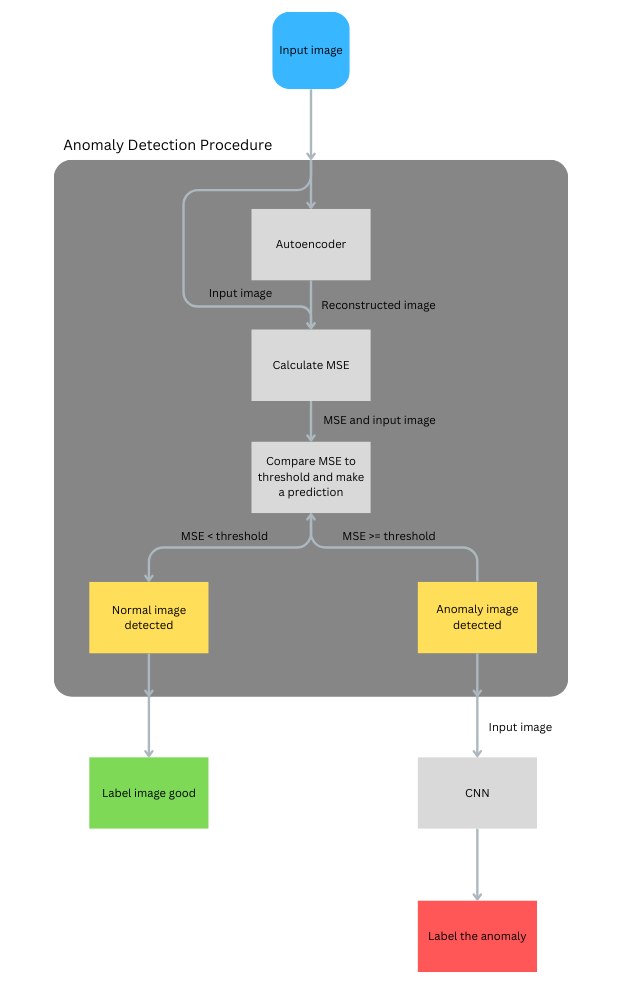
\includegraphics[scale=0.6]{src/images/machine_learning_pipeline.png}
    \caption{Machine learning pipeline visualized}
    \label{fig:ml_pipeline}
\end{figure}

\subsection{Autoencoder}
In order to reconstruct the original images we used a convolutional autoencoder. This type of autoencoder is well suited for image data as it can capture spatial information and learn hierarchical features. 

\subsubsection{Data preparation and Augmentation}

To train our autoencoder, we sort out the normal images from the dataset and use them as training data. We also create more training data by mirroring each image on the x-axis and also on the y-axis. Each one of the original images and the mirrored images are then rotate first 90 degrees, then 180 degrees and finally 270 degrees. This results in each original image getting transformed into 12 total different images.

\subsubsection{Implemention}

The autoencoder is implemented using TensorFlow Keras Model API with the following architecture:
\vspace{0.3cm}
\begin{python}
encoder_input = Input(shape=(image_size[0], image_size[1], 3))

# Encoding layers
x = Conv2D(32, (3, 3), activation="relu", padding="same")(encoder_input)
x = BatchNormalization()(x)
x = MaxPooling2D((2, 2), padding="same")(x)
x = Conv2D(32, (3, 3), activation="relu", padding="same")(x)
x = BatchNormalization()(x)
x = MaxPooling2D((2, 2), padding="same")(x)
x = Conv2D(32, (3, 3), activation="relu", padding="same")(x)

encoded_shape = x.shape[1:]

# Flatten layers
x = Flatten()(x)
flat_length = x.shape[1]
x = Dense(1024, activation="relu")(x)
x = Dense(flat_length, activation="relu")(x)
x = Reshape(encoded_shape)(x)

# Decoding layers
x = Conv2DTranspose(32, (3, 3), strides=2, activation="relu", padding="same")(x)
x = Conv2DTranspose(32, (3, 3), strides=2, activation="relu", padding="same")(x)
x = Conv2D(3, (3, 3), activation="sigmoid", padding="same")(x)
\end{python}

Three different convolutional layers, each followed by max pooling layers, are used to encode the input images. The encoded shape is then flattened and passed through two dense layers before reshaping it back to the encoded shape. The decoding layers consist of two transposed convolutional layers and a final convolutional layer that outputs the reconstructed image.
\par
We use ``ReLU'' as the activation function for each convolutional and dense layer, except for the final convolutional layer, where we use the ``Sigmoid'' activation function. 
\par
To compile the model, we use the ``Adam'' optimizer with a learning rate of $0.0005$ and mean-squared error as the loss function. We also define two different callback-functions that monitors validation loss:
\begin{python}
reduce_lr = ReduceLROnPlateau(monitor="val_loss", factor=0.2, patience=3, min_delta=0.0005)
early_stop = EarlyStopping(monitor="val_loss", patience=5, min_delta=0.0002, restore_best_weights=True)
\end{python}

\subsection{Anomaly detection procedure}

Our design of a anomaly detection is based around the reconstruction error of the autoencoder. To measure reconstruction we use the same method as for our loss function in training the autoencoder, mean-squared error. To set a threshold for when an image is to be consider an anomaly, we calculate the mean-squared error for normal images and also for anomalies. We then set the avarage value of the highest mse of the normal images and the lowest value for the anomalies as the threshold.
\par
When the autoencoder is trained and the threshold is set, we make predictions on test data that the autoencoder has not seen before. If the mse of an image is above the threshold, we consider it an anomaly and pass it to the CNN for classification.

\subsection{CNN}

\subsubsection{Introducing noise}
To ensure model robustness in real-world conditions, we introduced two types of noise to the images: Gaussian noise and Salt and Pepper noise. 
Gaussian noise simulates random intensity variations that might occur due to poor lighting or sensor noise, while Salt and Pepper noise represents random white and black pixels that could appear due to dead pixels or transmission errors.
Additionally, we introduced noise by flipping and rotating images, which simulates diffrent camera angels and orientations.

\begin{figure}[H]
    \centering
    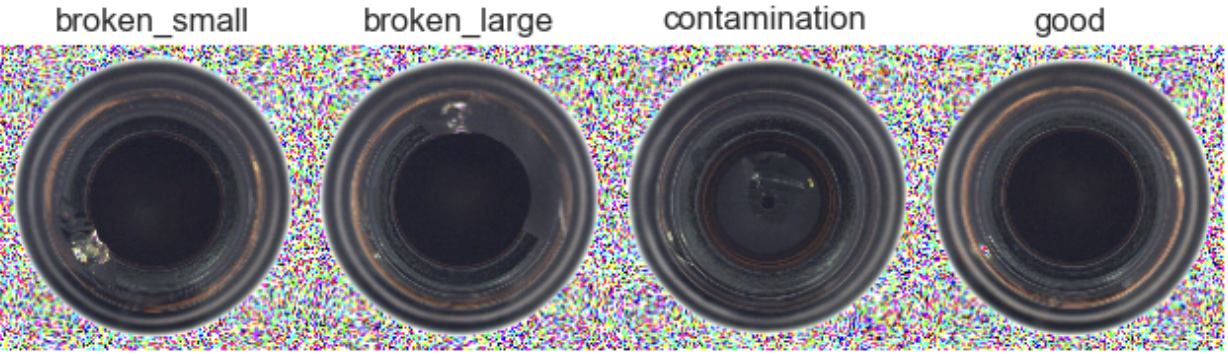
\includegraphics[scale=0.55]{src/images/dataset_w_gnoise.png}
    \caption{Images with Gaussian noise.}
    \label{fig:Gnoise}
\end{figure}
\begin{figure}[H]
    \centering
    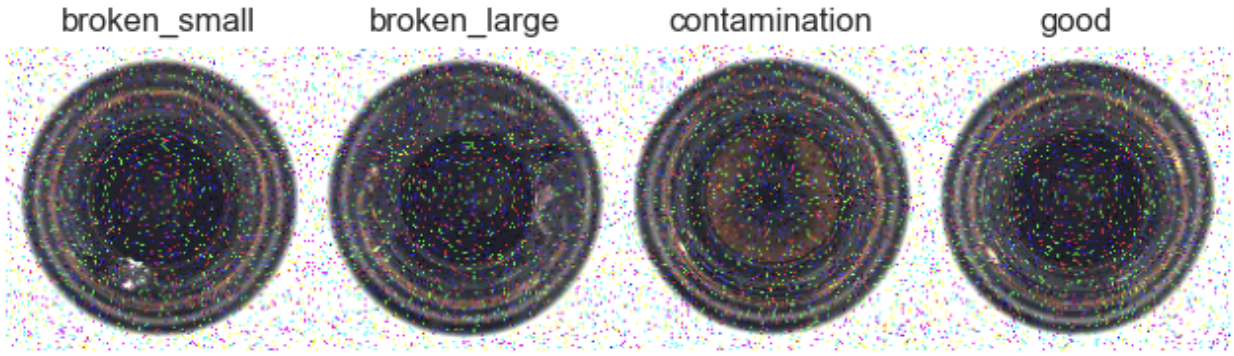
\includegraphics[scale=0.55]{src/images/dataset_w_snp.png}
    \caption{Images with Salt and Pepper noise.}
    \label{fig:snpnoise}
\end{figure}

\subsubsection{Implemention}
The CNN model is implemented using TensorFlow's Sequential API with the following architecture:
\vspace{0.3cm}
\begin{python}
model = models.Sequential([
    layers.InputLayer(shape=(150, 150, 3)), 
    layers.Conv2D(32, (3, 3), activation='relu', padding='same', strides=(2, 2)),
    layers.MaxPooling2D((2, 2)),
    layers.Conv2D(64, (3, 3), activation='relu', padding='same', strides=(2, 2)),
    layers.MaxPooling2D((2, 2)),
    layers.Conv2D(128, (3, 3), activation='relu', padding='same', strides=(2, 2)),
    layers.MaxPooling2D((2, 2)),
    layers.Flatten(),
    layers.Dense(128, activation='relu'),
    layers.Dense(4, activation='softmax')
])
model.compile(
    optimizer='adam',
    loss='categorical_crossentropy',
    metrics=['accuracy']
)
\end{python}

The model consists of three convolutional layers, each followed by max pooling layers, and two dense layers for classification. The input images are 150x150 pixels with 3 color channels.

